\section{Materials and Methods}


%%%%%%%%%%%%%%%%%%%%%%%%%%%%%
% SECTION 3.1 BELOW
%%%%%%%%%%%%%%%%%%%%%%%%%%%%%


\subsection{Model-development workflow}

\subsubsection{Starting point and relation to previous EWS FEM work}

This project was developed in the context of previous internal EWS finite element modelling work. Earlier EWS models provided a useful methodological starting point for breast geometry parameterisation, soft-tissue material assumptions, dynamic loading and displacement-based evaluation \cite{EngelsEWSReport, StormEWSReport}. These previous projects were used as engineering reference material and as a comparison point for modelling choices. They were not used as validation datasets for the current COMSOL model.

The present project develops a separate COMSOL-based modelling route. The motivation for this route was to improve control over constructive geometry, region definitions, model variants and post-processing while keeping the workflow reproducible. This was especially relevant because the project aimed to investigate the influence of individual anatomical and mechanical components, including chestwall shape, fibroglandular tissue distribution, skin representation, Cooper-ligament support approximation and tumor inclusion. Additional context on the previous EWS FEM work is provided in Appendix~\ref{sec:appendix_previous_ews_fem_work}, while the current repository structure is summarised in Appendix~\ref{sec:appendix_current_repository}.

\subsubsection{COMSOL-based workflow}

The finite element model was implemented in COMSOL Multiphysics and controlled using a Python-based source-case workflow \cite{COMSOLMultiphysicsWebsite}. Each model variant was defined by a case configuration file containing the main geometry, material, loading and evaluation settings. These settings were used to generate a consistent COMSOL model definition, including the required geometry operations, material assignments, selections, study settings and post-processing outputs. An overview of the workflow is shown in Figure~\ref{fig:comsol_pipeline_overview}.

\begin{figure}[H]
\centering
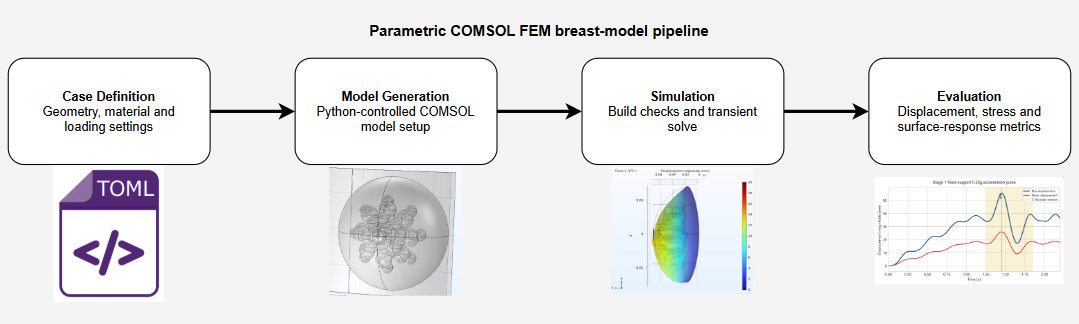
\includegraphics[width=0.95\linewidth]{Figures/M&M/model_overviews/Report_pipeline_overview.png}
\caption{Overview of the COMSOL-based model-development workflow. Case definitions specify the main geometry, material and loading settings. These settings are used by the Python-controlled workflow to generate the COMSOL model, perform build and solve steps, and export compact evaluation outputs for comparison.}
\label{fig:comsol_pipeline_overview}
\end{figure}

The purpose of this workflow was to make model changes traceable. Instead of manually modifying a COMSOL model for each comparison, the relevant modelling assumptions were stored in version-controlled case definitions. This allowed related model variants to be generated from a consistent structure and made it easier to identify which modelling change was responsible for a difference in the simulated displacement or stress response. The project repository contains the implementation of the Python workflow, the active TOML case definitions and the compact evaluation outputs used for the comparisons \cite{KuijpersEWSComsolGitHub}. These case definitions were used to keep the modelling assumptions for each variant traceable without relying on manual edits to a single COMSOL model file.

\subsubsection{Model-development strategy}

The model was developed by adding and testing one modelling component at a time. The development was organised around six main modelling themes: dynamic excitation, posterior chestwall geometry, internal fibroglandular tissue distribution, outer-shape variation, mechanical support representation and tumor sensitivity. This structure was used to reduce the risk of interpreting multiple model changes at once.

The first part of the workflow focused on establishing a stable dynamic input and a controlled anatomical reference geometry. The posterior support was then refined using a curved chestwall representation, followed by a more detailed fibroglandular tissue distribution. After this anatomical route was established, additional model variants were used to investigate outer-shape asymmetry, Cooper-ligament support approximations, and skin and material sensitivity. Tumor sensitivity was treated as a separate final extension of the workflow. In this extension, spherical tumor-overlay definitions were prepared for different sizes and locations to test whether local stiffness inclusions could be added consistently to the existing COMSOL model. The overall model-development route is summarised in Figure~\ref{fig:model_development_route}.

\begin{figure}[H]
\centering
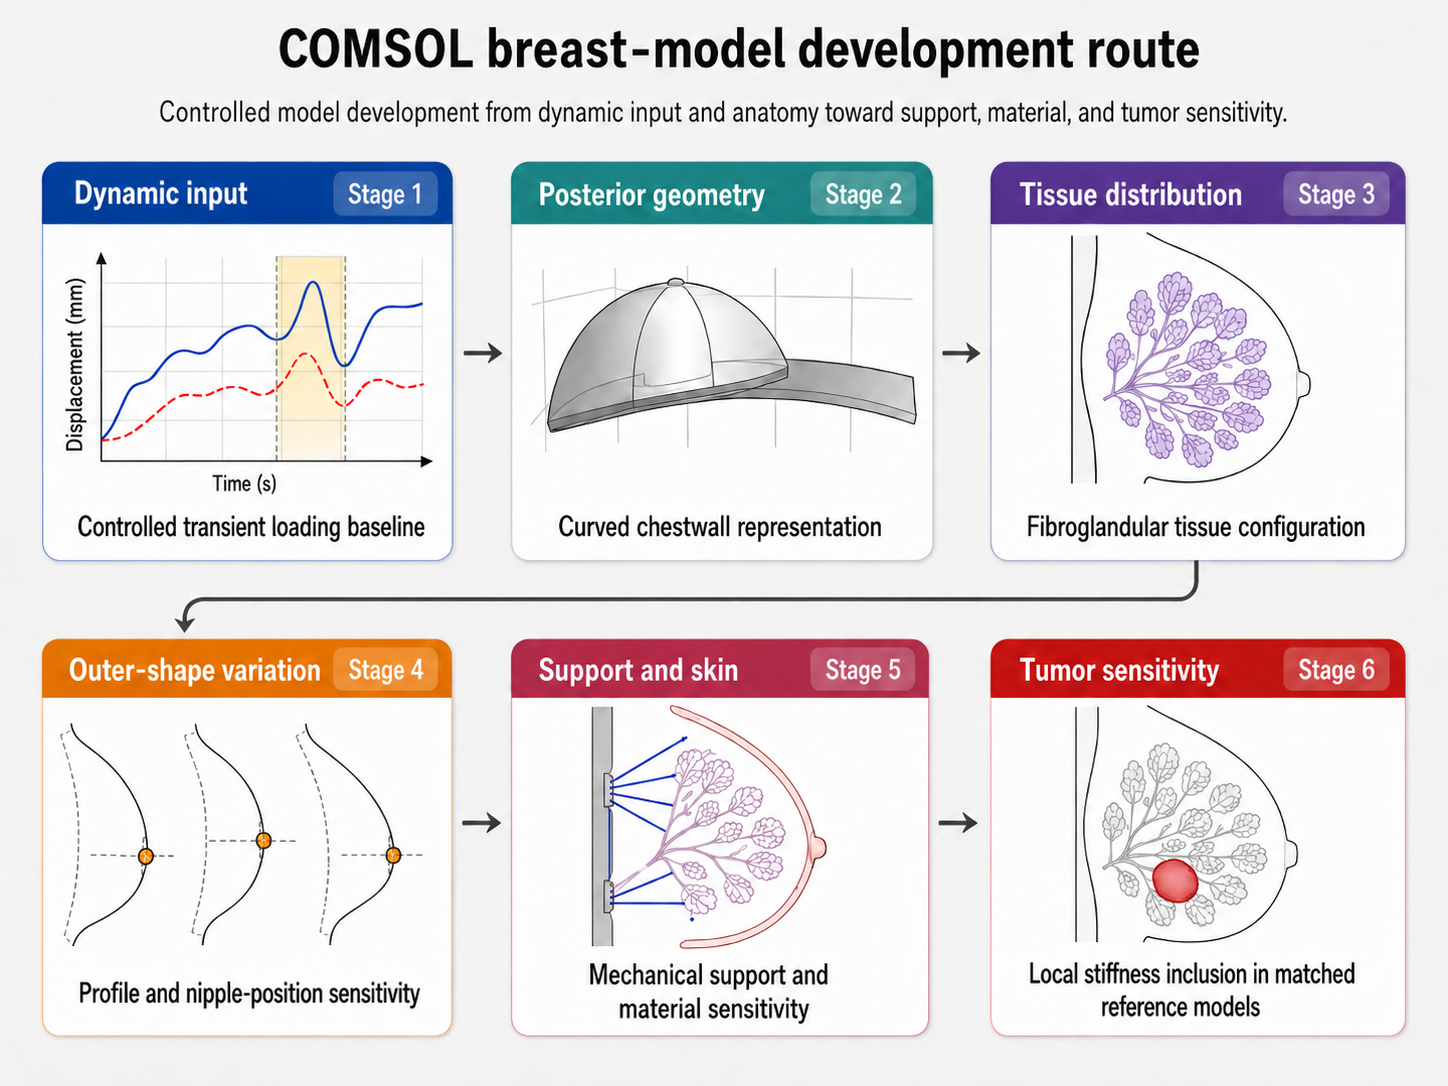
\includegraphics[width=0.95\linewidth]{Figures/M&M/model_overviews/report_staged_model_overview.png}
\caption{Schematic overview of the COMSOL breast-model development route used in this project. The workflow progresses from dynamic input and anatomical model definition toward outer-shape variation, support and skin sensitivity, and tumor sensitivity, allowing individual modelling components to be investigated in a controlled manner.}
\label{fig:model_development_route}
\end{figure}

Not all model variants had the same interpretation status. Some cases were used as controlled reference models for quantitative comparison, whereas others were used as exploratory checks for numerical stability, geometry construction or sensitivity to modelling assumptions. This distinction is important because the aim of the project was not to validate a final patient-specific diagnostic model, but to construct a reproducible COMSOL FEM workflow and to identify which modelling components have a measurable influence on the simulated breast deformation response.


%%%%%%%%%%%%%%%%%%%%%%%%%%%%%
% SECTION 3.2 BELOW
%%%%%%%%%%%%%%%%%%%%%%%%%%%%%


\subsection{Anatomical model definition}
\label{sec:anatomical_model_definition}

The anatomical model was defined as a parametrised breast representation rather than as a reconstruction of one individual patient. This choice reflects the aim of the EWS modelling workflow to generate controlled breast-model variants that can be used to study how anatomy, tissue distribution, material assumptions and tumor properties affect the simulated surface deformation response. In the longer term, such a parametrised modelling route could support the generation of synthetic deformation data for algorithm development and AI training, provided that the simulated responses are sufficiently well understood and validated. Patient-specific breast geometries remain important for clinical modelling applications \cite{Samani2001,Hsu2011,Mazier2024}, but the present work focuses on building a reproducible model-development platform that can later be extended toward broader anatomical variation and more patient-specific inputs.

In this section, the anatomical definition is limited to the geometric and tissue-layout components of the model. This includes the parametrised breast envelope, posterior chestwall representation, fibroglandular tissue distribution, and controlled outer-shape and nipple-position variations. Anatomically motivated components that were implemented mainly through material or support definitions, such as the skin layer, Cooper-ligament support approximation and tumor inclusion, are described in Section~\ref{sec:mechanical_model_definition}.

\subsubsection{Parametrised breast geometry and reference volume}
\label{sec:parametrised_breast_geometry}

The overall breast shape was generated from the TOML case-definition parameters used by the COMSOL pipeline. For the selected anatomical route, the model used a characteristic radius of 70~mm, an elliptic outer profile, an anterior projection scale of 1.08 and a superior-pole scale of 0.98. The radius sets the global model scale, while the profile and scaling factors adjust the anterior projection and upper-breast shape. These parameters were selected as representative model-construction settings for the reference geometry.

The reference volume was chosen by comparing the generated COMSOL geometry with literature values for breast-volume measurement and with an internal Catharina Hospital dataset of 100 manually delineated breast volumes \cite{Stahl2023,Yoo2013,Nie2010SkinRemoval,Choppin2016}. The details of this comparison are provided in Appendix~\ref{sec:appendix_breast_volume_reference}. Because breast-volume estimates depend on measurement method, patient position and boundary definition, the selected volume was not treated as a single population average, but as a defensible reference size for controlled model development.

After the COMSOL geometry operations, including posterior support construction and volume-preserving compensation, the selected anatomical route produced a breast volume of $\sim$585~mL. This value is within the lower-mid range of the internal dataset and is consistent with the literature-based volume context. It was therefore used as a controlled reference volume for the main matched comparisons. Keeping this volume fixed prevented later changes in tissue distribution, asymmetry, support representation or tumor inclusion from being combined with a change in overall breast size.

\subsubsection{Posterior chestwall representation}
\label{sec:posterior_chestwall_representation}

The posterior boundary of the breast was represented by a simplified chestwall support geometry. This support was not intended as a full anatomical reconstruction of the thoracic wall or pectoral region, but as a controlled posterior interface that better reflects the curved support on which the breast rests than the flat chestwall used in earlier internal EWS modelling work. Curved posterior support is also consistent with breast FEM literature, where the breast is commonly modelled relative to the thoracic wall, pectoral region or posterior support boundary \cite{Hsu2011,Mazier2024}.

In the selected reference route, the posterior support was implemented as a transverse curved support geometry with volume-preserving compensation, as shown in Figure~\ref{fig:chestwall_reference_geometry}. In the COMSOL case definition, this route used the support mode \texttt{transverse\_vp}, a transverse curve depth of 21~mm and a chestwall-curve centre offset of +55~mm in the COMSOL $x$-direction. The posterior support was generated using a \texttt{cylinder\_band} geometry, such that the chestwall shape could be adjusted through the curvature depth and offset parameters. A positive offset represents the selected left-breast orientation used in this report route, while the same construction can be mirrored using a negative offset for a right-breast orientation.

\begin{figure}[H]
\centering
\begin{subfigure}{0.48\linewidth}
\centering
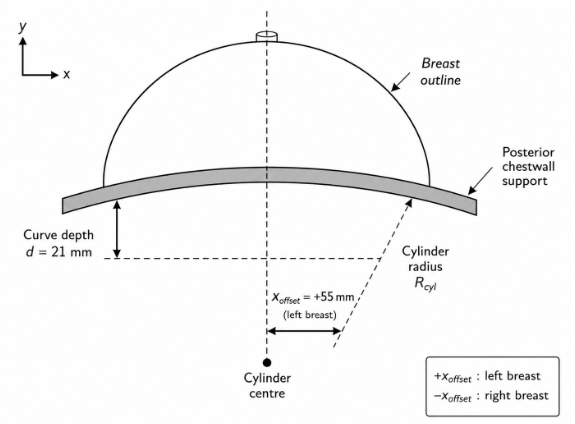
\includegraphics[width=\linewidth]{Figures/M&M/Schematic_chestwall_parameters.png}
\caption{Schematic top view}
\end{subfigure}
\hfill
\begin{subfigure}{0.48\linewidth}
\centering
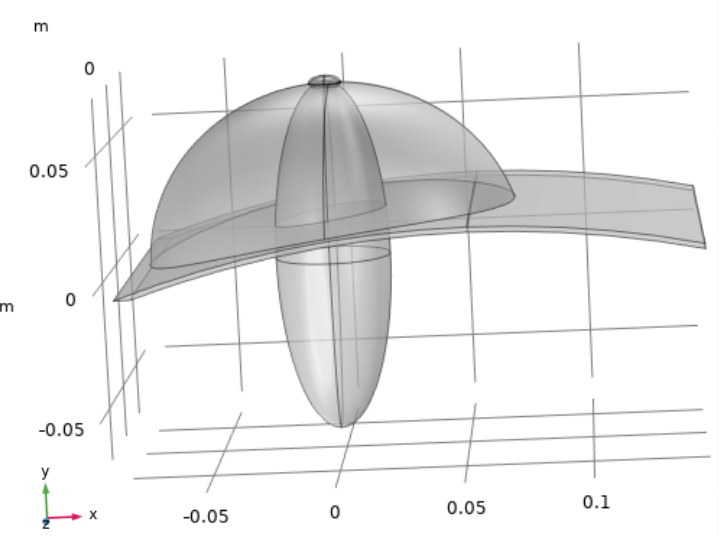
\includegraphics[width=\linewidth]{Figures/M&M/Superior_chestwallcurve.png}
\caption{COMSOL-rendered superior view}
\end{subfigure}
\caption{Posterior chestwall representation used in the selected reference route. The schematic view illustrates the transverse curved support geometry, including the curvature depth and the $x$-offset of the cylinder centre. The COMSOL-rendered view shows the corresponding curved posterior support geometry for the selected $+55~\mathrm{mm}$ chestwall-offset configuration.}
\label{fig:chestwall_reference_geometry}
\end{figure}

Superior--inferior curvature can also be combined with the transverse support geometry in the pipeline. However, this additional curvature was not retained in the selected reference baseline because the transverse curvature represented the dominant anatomical refinement compared with the earlier flat chestwall, while exploratory COMSOL checks showed only a limited additional effect from the superior--inferior component. Excluding this extra curvature also kept the reference geometry simpler and more stable for the matched comparisons. To preserve geometric consistency across parameter choices, the nipple-related helper geometry and anterior glandular alignment were updated automatically relative to the selected chestwall shape using projected-normal alignment.


\subsubsection{Fibroglandular tissue distribution}
\label{sec:fibroglandular_tissue_distribution}

The fibroglandular tissue representation was refined from a simple internal region toward a more structured lobule-based distribution. This step was included to make the internal tissue layout more anatomically realistic, because breast tissue is heterogeneous and internal tissue composition can influence the simulated deformation response \cite{Chen2024,Mazier2024}.

The selected reference route was guided mainly by the multi-component breast-model approach described by Chen et al. \cite{Chen2024}. In the COMSOL implementation, the fibroglandular region was generated using the \texttt{chen\_2024\_template\_lobes} mode. The reference configuration used 12 lobules, divided into 4 inner and 8 outer lobules, with duct-like components directed toward the nipple, a subareolar core and a subareolar bridge. A lateral view of the reference configuration is shown in Figure~\ref{fig:fibroglandular_reference_lateral}.

Three spread variants were retained: compact, reference and wide. These variants changed the spatial spread of the lobules while keeping the selected Stage~2 chestwall geometry and the same general model setup. The reference spread was used as the main anatomical route for later comparisons, while the compact and wide variants were used to check the geometric effect of the assumed fibroglandular spread. The compact and wide variants are shown in Figure~\ref{fig:fibroglandular_spread_variants}.

The current reference model had a total breast volume of $\sim$585~mL and used a glandular fraction of $\sim$24.3\%, corresponding to a glandular volume of $\sim$142.2~mL. This value was considered acceptable for the reference route after comparison with literature on volumetric breast density and fibroglandular tissue quantification \cite{Sartor2016,Nie2010,Lu2012}. Because volumetric fibroglandular fraction is not directly equivalent to projected mammographic density or to the Breast Imaging Reporting and Data System (BI-RADS) breast-composition categories, the literature context is summarised separately in Appendix~\ref{sec:appendix_glandular_fraction_reference} \cite{ACRBIRADS}. The resulting reference and spread-variation layouts are shown in Figure~\ref{fig:fibroglandular_distribution_variants}.

\begin{figure}[H]
\centering
\begin{subfigure}{0.32\linewidth}
\centering
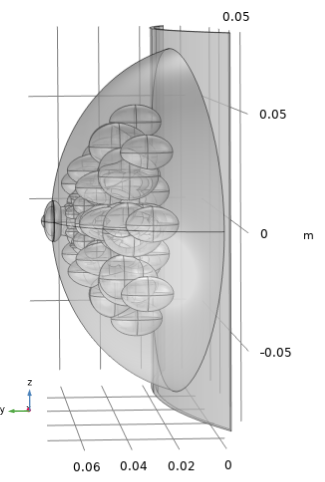
\includegraphics[width=\linewidth,height=0.24\textheight,keepaspectratio]{Figures/M&M/leftantroir_view_gland.png}
\caption{Reference lateral view}
\label{fig:fibroglandular_reference_lateral}
\end{subfigure}
\hfill
\begin{subfigure}{0.64\linewidth}
\centering
\begin{minipage}{0.48\linewidth}
\centering
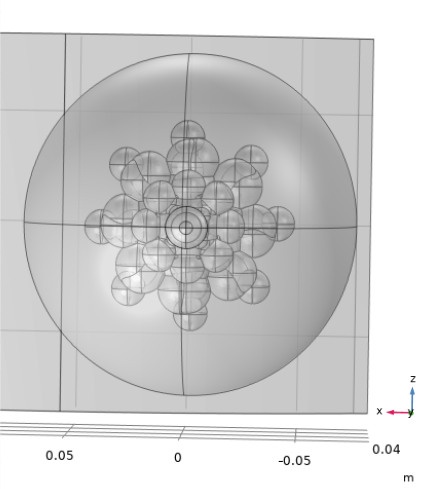
\includegraphics[width=\linewidth]{Figures/M&M/compact_spread.png}
\end{minipage}
\hfill
\begin{minipage}{0.48\linewidth}
\centering
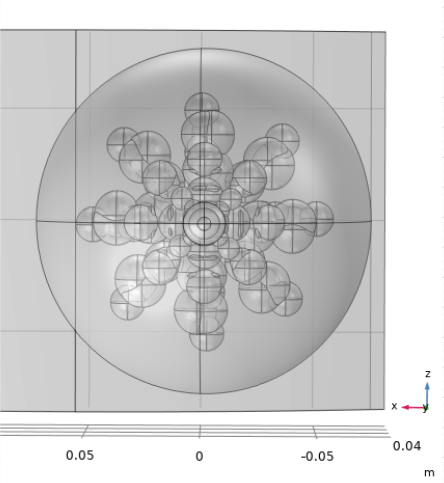
\includegraphics[width=\linewidth]{Figures/M&M/wide_spread.png}
\end{minipage}
\caption{Compact (left) and wide (right) anterior views}
\label{fig:fibroglandular_spread_variants}
\end{subfigure}

\caption{COMSOL-rendered fibroglandular tissue configurations used in the Stage~3 anatomical route. The reference lateral view shows the chestwall-aware lobule and duct structure inside the selected $+55~\mathrm{mm}$ chestwall-offset geometry. The compact and wide anterior views illustrate the spread variants used to evaluate the effect of fibroglandular spatial distribution.}
\label{fig:fibroglandular_distribution_variants}
\end{figure}

\subsubsection{Outer-shape and nipple-position variations}
\label{outer_shape_nipple_variations}

Outer-shape and nipple-position variations were included because breast size, shape and left--right symmetry vary substantially between individuals \cite{Stahl2023,Mazier2024}. For an EWS-oriented model, this is relevant because surface shape and nipple position influence both the visible breast surface and the interpretation of local displacement or landmark motion.

Stage~4 was therefore used to test controlled geometry variations on top of the selected Stage~2 chestwall geometry and Stage~3 fibroglandular reference. In the COMSOL case definitions, the outer breast shape can be scaled in width and height, while the nipple position can be shifted over the breast surface in the $x$- and $z$-directions. Examples of these geometry variations are shown in Figure~\ref{outer_shape_nipple_variation_examples}.

For nipple-position variations, the associated lobules, ducts, subareolar core and bridge were updated relative to the final nipple axis, so that the internal fibroglandular layout remained coupled to the shifted nipple position. These cases were used as controlled geometry-sensitivity previews and should not be interpreted as patient-specific asymmetry reconstructions.


\begin{figure}[H]
\centering
\begin{subfigure}{0.32\linewidth}
\centering
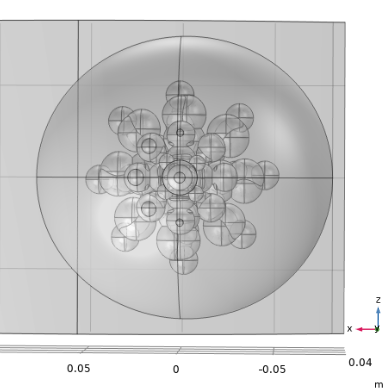
\includegraphics[width=\linewidth]{Figures/M&M/scaling.png}
\caption{Profile scaling (widening)}
\label{stage4_profile_scaling_panel}
\end{subfigure}
\hfill
\begin{subfigure}{0.32\linewidth}
\centering
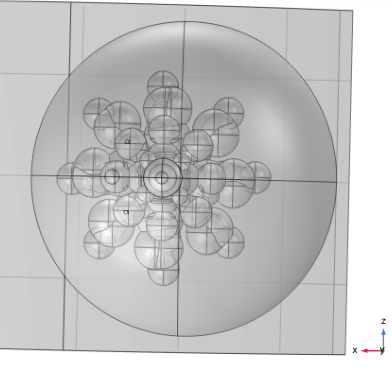
\includegraphics[width=\linewidth]{Figures/M&M/lateral_nipple.png}
\caption{Lateral nipple shift}
\label{stage4_lateral_nipple_shift_panel}
\end{subfigure}
\hfill
\begin{subfigure}{0.32\linewidth}
\centering
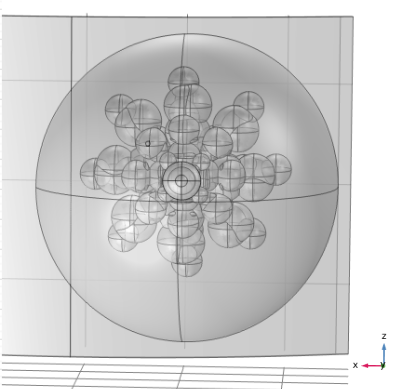
\includegraphics[width=\linewidth]{Figures/M&M/superior_nipple.png}
\caption{Superior nipple shift}
\label{stage4_superior_nipple_shift_panel}
\end{subfigure}

\caption{COMSOL-rendered examples of the outer-shape and nipple-position variation cases used in Stage~4. The cases test controlled changes in breast profile and nipple position while preserving the selected Stage~2 chestwall route and Stage~3 fibroglandular reference.}
\label{outer_shape_nipple_variation_examples}
\end{figure}




%%%%%%%%%%%%%%%%%%%%%%%%%%%%%
% SECTION 3.3 BELOW
%%%%%%%%%%%%%%%%%%%%%%%%%%%%%


\subsection{Mechanical model definition}
\label{sec:mechanical_model_definition}

The mechanical model defines how the anatomical regions described in Section~\ref{sec:anatomical_model_definition} were assigned material behaviour and mechanical support assumptions in COMSOL. The workflow was organised into separate material and support routes, so that the influence of individual modelling choices, including tissue stiffness, skin representation, Cooper-ligament support and tumor inclusion, could be evaluated independently from the anatomical geometry. This separation allowed the mechanical contribution of each model component to be tested without redefining the underlying segmented breast shape.

\subsubsection{Constitutive material model}
\label{constitutive_material_model}

Breast tissue was modelled as a soft, nearly incompressible material. This is consistent with common breast FEM practice, although reported mechanical properties vary substantially between studies because of differences in measurement protocol, preload, strain level, tissue type and constitutive model \cite{Samani2007,Ramiao2016,Goodbrake2022,Teixeira2023}. In the COMSOL source-case definition, adipose, fibroglandular, skin and tumor materials were parameterised using density, bulk modulus $K$ and two Mooney--Rivlin-type coefficients, $C_{10}$ and $C_{01}$. Related Mooney--Rivlin-type soft-tissue material descriptions were also used in previous internal EWS/FEBio modelling work, which served as historical reference material for the current COMSOL route \cite{EngelsEWSReport,StormEWSReport}.

The source material parameterisation can be written in terms of a deviatoric Mooney--Rivlin strain-energy density with an additional volumetric contribution \cite{Mooney1940,Rivlin1948},

\begin{equation}
W
=
C_{10}\left(\bar{I}_{1}-3\right)
+
C_{01}\left(\bar{I}_{2}-3\right)
+
W_{\mathrm{vol}}\left(J;K\right).
\label{mooney_rivlin_strain_energy_density}
\end{equation}

Here, $\bar{I}_{1}$ and $\bar{I}_{2}$ are the modified invariants, $J$ is the volume ratio and the volumetric part is controlled by the bulk modulus $K$. Equation~\ref{mooney_rivlin_strain_energy_density} describes the source material parameterisation used in the workflow. It should not be interpreted as a full derivation of the exact volumetric penalty formulation used internally by COMSOL.

For stiffness-scale interpretation, and for the effective small-strain material route used where the COMSOL implementation requires linear-elastic quantities, the Mooney--Rivlin source parameters were mapped to equivalent small-strain elastic constants using:

\begin{equation}
G_{0}
=
2\left(C_{10}+C_{01}\right),
\label{small_strain_shear_modulus_from_mooney_rivlin}
\end{equation}

\begin{equation}
E
=
\frac{9KG_{0}}{3K+G_{0}},
\label{small_strain_youngs_modulus_from_bulk_and_shear}
\end{equation}

and

\begin{equation}
\nu
=
\frac{3K-2G_{0}}{2\left(3K+G_{0}\right)}.
\label{small_strain_poisson_ratio_from_bulk_and_shear}
\end{equation}

The coefficients $C_{10}$ and $C_{01}$ determine how strongly the Mooney--Rivlin material resists shape change at small deformation. Their sum gives the small-strain shear modulus $G_{0}$. This shear modulus was then combined with the bulk modulus $K$, which controls resistance to volume change, to obtain an equivalent Young's modulus $E$ and Poisson's ratio $\nu$ for small-strain interpretation. Because soft breast tissue was treated as nearly incompressible, $K$ was chosen much larger than $G_{0}$, resulting in $\nu$ close to $0.5$.

For nearly incompressible behaviour, where $K$ is much larger than $G_{0}$, this reduces approximately to

\begin{equation}
E
\approx
3G_{0}
=
6\left(C_{10}+C_{01}\right).
\label{nearly_incompressible_stiffness_scale}
\end{equation}

The resulting stiffness value $E$ was therefore reported as a small-strain equivalent stiffness, allowing the material sets to be compared more directly with each other and with literature values commonly reported in terms of Young's modulus. It does not replace the original Mooney--Rivlin source-parameter definition. The posterior chestwall support was represented separately using a linear elastic surrogate material with $E=10~\mathrm{kPa}$ and $\nu=0.49$.



\subsubsection{Material parameter sets}
\label{material_parameter_sets}

The material parameter sets were defined to support both a main reference configuration and additional stiffness-sensitivity cases. The reference values were selected from the literature comparison and internal model-justification notes, with the aim of keeping the adipose and fibroglandular stiffnesses within the low-kPa range commonly used for breast soft-tissue FEM models \cite{Samani2007,Ramiao2016,Goodbrake2022,Teixeira2023}. A summary of the literature values considered during parameter selection is provided in Appendix~\ref{appendix_material_parameter_literature_summary}.

In addition to the reference set, lower- and higher-stiffness variants were tested using the same anatomical geometry and boundary-condition route. These variants were included to evaluate the sensitivity of the simulated mechanical response to the selected material stiffness.

The main material definitions used in the COMSOL model-development workflow are summarised in Table~\ref{material_parameter_sets_table}. The listed Young's modulus values are included as small-strain equivalent stiffness values, so that the material scale can be compared more easily across parameter sets and with literature values reported in terms of Young's modulus.

\begin{table}[H]
\centering
\small
\caption{Main material parameters used in the COMSOL model-development workflow.}
\label{material_parameter_sets_table}
\begin{tabular}{p{0.23\linewidth} p{0.12\linewidth} p{0.16\linewidth} p{0.28\linewidth} p{0.13\linewidth}}
\toprule
Component 
& Density 
& Bulk / elastic setting 
& Material coefficients 
& Stiffness scale \\
\midrule
Adipose tissue 
& $950~\mathrm{kg\,m^{-3}}$ 
& $K=425~\mathrm{kPa}$ 
& $C_{10}=310~\mathrm{Pa}$; $C_{01}=300~\mathrm{Pa}$ 
& $E\approx3.66~\mathrm{kPa}$ \\

Fibroglandular tissue 
& $1070~\mathrm{kg\,m^{-3}}$ 
& $K=425~\mathrm{kPa}$ 
& $C_{10}=833~\mathrm{Pa}$; $C_{01}=833~\mathrm{Pa}$ 
& $E\approx10.0~\mathrm{kPa}$ \\

Skin layer 
& $1100~\mathrm{kg\,m^{-3}}$ 
& $K=8.33~\mathrm{MPa}$ 
& $C_{10}=41667~\mathrm{Pa}$; $C_{01}=41667~\mathrm{Pa}$ 
& $E\approx500~\mathrm{kPa}$ \\

Hard tumor overlay case
& $1079~\mathrm{kg\,m^{-3}}$
& $K=425~\mathrm{kPa}$ 
& $C_{10}=8333~\mathrm{Pa}$; $C_{01}=8333~\mathrm{Pa}$ 
& $E\approx100~\mathrm{kPa}$ \\

Chestwall support 
& $1050~\mathrm{kg\,m^{-3}}$ 
& $E=10~\mathrm{kPa}$; $\nu=0.49$ 
& Linear elastic support material 
& $E=10~\mathrm{kPa}$ \\
\bottomrule
\end{tabular}
\end{table}

\subsubsection{Volumetric skin representation}
\label{volumetric_skin_representation}

The skin was treated as a separate mechanical component because its stiffness can be substantially higher than that of the internal adipose and fibroglandular tissues, making it relevant for whole-breast deformation \cite{Chen2025,Teixeira2023}. During model development, both surface-based shell and volumetric solid-layer representations were considered. Shell-based skin descriptions were used in previous internal EWS/FEBio work \cite{EngelsEWSReport,StormEWSReport} and are also used in breast finite-element models reported in the literature \cite{Chen2025}. A volumetric layer was retained for the COMSOL route because it allowed the skin to be defined through the same material parameter workflow as the internal breast tissues.

In the active skin-enabled cases, the volumetric skin layer was assigned a thickness of $1.5~\mathrm{mm}$. This value is consistent with reported breast skin thickness measurements and modelling assumptions in the literature, where average values around $1.45$--$1.55~\mathrm{mm}$ and modelled skin thicknesses in the same range have been reported \cite{Huang2008,Sutradhar2012,Hsu2011,Chen2025}. The skin material used the density, bulk modulus and Mooney--Rivlin-type coefficients listed in Table~\ref{material_parameter_sets_table}.

Because reported skin stiffness values differ substantially between studies and depend on the measurement method and modelling assumptions, the skin stiffness was also varied in sensitivity cases \cite{Ramiao2016,Teixeira2023}. These variants were compared with the no-skin model to evaluate the mechanical influence of adding a distinct skin layer. Earlier COMSOL shell/scaffold skin attempts were not retained as the main implementation route because they produced unrealistic breast-surface behaviour in the generated models and were less straightforward to control than the volumetric solid-layer implementation.

\subsubsection{Cooper-ligament support approximation}
\label{cooper_ligament_support_approximation}

Cooper-ligament support was represented as a simplified mechanical support contribution rather than as a reconstructed anatomical ligament network. Similar reduced support representations are common in breast finite-element modelling, where fibrous structures such as Cooper's ligaments are often approximated because they are difficult to segment and assign patient-specific material properties \cite{Chen2025,Teixeira2023,Mazier2024}. In the current COMSOL route, the support contribution was implemented through displacement-proportional restoring tractions on selected anterior support regions. This provided a separate model-development route for testing the effect of Cooper-like support on the simulated breast response.

Three support-selection variants were implemented. The first connected the nipple-region support to the posterior chestwall direction, the second applied support between skin and glandular regions, and the third used a denser skin-to-glandular support selection. These variants were used to compare different simplified approximations of anterior fibrous support without reconstructing a full anatomical Cooper-ligament network.

The support scale was defined from an assumed ligament stiffness, an active area fraction and a reference length,

\begin{equation}
k_{\mathrm{Cooper}}
=
\frac{E_{\mathrm{Cooper}} f_{\mathrm{area}}}{L_{\mathrm{ref}}}.
\label{cooper_support_scale_from_area_fraction}
\end{equation}

The active restoring traction was applied in the global anterior--posterior direction as

\begin{equation}
t_{y}
=
-k_{y}v,
\label{cooper_y_restoring_traction}
\end{equation}

where $v$ is the COMSOL displacement component in the $y$-direction and $k_{y}$ is the corresponding support scale. For the selection-specific support regions, the implemented scaling factors were

\begin{equation}
k_{\mathrm{skin}}
=
0.65k_{\mathrm{Cooper}},
\qquad
k_{\mathrm{gland}}
=
0.45k_{\mathrm{Cooper}},
\qquad
k_{\mathrm{nipple}}
=
0.20k_{\mathrm{Cooper}}.
\label{cooper_selection_specific_support_scales}
\end{equation}

The default support scale used $E_{\mathrm{Cooper}}=5.8~\mathrm{MPa}$, $f_{\mathrm{area}}=0.12$ and $L_{\mathrm{ref}}=0.04~\mathrm{m}$, giving $k_{\mathrm{Cooper}}=17.4\times10^{6}~\mathrm{N\,m^{-3}}$. Lower and higher area-fraction variants were also prepared as sensitivity cases.

Because reported Cooper-ligament properties and effective whole-breast support values differ substantially between studies, the current values should be interpreted as support-strength parameters rather than direct anatomical ligament measurements \cite{Teixeira2023,Chen2025}. The no-Cooper model was retained as the comparison route, while the Cooper-support variants were implemented to evaluate the additional mechanical influence of simplified Cooper-like support.

\subsubsection{Tumor representation}
\label{tumor_representation}

Tumor inclusion was implemented as an analytic spherical material overlay inside the existing breast volume. The tumor was therefore not defined as a separate COMSOL geometry domain, but as a local modification of the material density and stiffness parameters inside the existing adipose and fibroglandular domains.

The tumor mask was defined as

\begin{equation}
m_{\mathrm{tumor}}(\mathbf{x})
=
\begin{cases}
1, & \left\|\mathbf{x}-\mathbf{x}_{\mathrm{tumor}}\right\| \leq r_{\mathrm{tumor}}, \\
0, & \left\|\mathbf{x}-\mathbf{x}_{\mathrm{tumor}}\right\| > r_{\mathrm{tumor}}.
\end{cases}
\label{tumor_spherical_material_overlay_mask}
\end{equation}

Here, $\mathbf{x}_{\mathrm{tumor}}$ is the tumor centre and $r_{\mathrm{tumor}}$ is the tumor radius. In the COMSOL implementation, this corresponds to the scalar variable \texttt{tumor\_mask}, which is equal to one inside the spherical overlay and zero outside it.

The local effective material properties were then modified using the tumor mask. For a surrounding tissue with base density $\rho$, base Young's modulus $E$ and base Mooney--Rivlin coefficients $C_{10}$ and $C_{01}$, the effective properties were defined as

\begin{equation}
\rho_{\mathrm{eff}}
=
\rho
+
m_{\mathrm{tumor}}\left(\rho_{\mathrm{tumor}}-\rho\right),
\label{tumor_effective_density}
\end{equation}

\begin{equation}
E_{\mathrm{eff}}
=
E
+
m_{\mathrm{tumor}}\left(E_{\mathrm{tumor}}-E\right),
\label{tumor_effective_youngs_modulus}
\end{equation}

\begin{equation}
C_{10,\mathrm{eff}}
=
C_{10}
+
m_{\mathrm{tumor}}\Delta C_{10,\mathrm{tumor}},
\label{tumor_effective_c10_coefficient}
\end{equation}

and

\begin{equation}
C_{01,\mathrm{eff}}
=
C_{01}
+
m_{\mathrm{tumor}}\Delta C_{01,\mathrm{tumor}}.
\label{tumor_effective_c01_coefficient}
\end{equation}

The current tumor material settings include both modest stiffness-contrast cases and a harder diagnostic-contrast case. Because the Early Warning Scan is aimed at detecting malignant breast tumors, the harder tumor-overlay setting was included to test a clear local stiffness contrast relative to normal breast tissue. In this high-contrast setting, the analytic overlay used $E_{\mathrm{tumor}}=100~\mathrm{kPa}$ together with local Mooney--Rivlin coefficient increments of $\Delta C_{10,\mathrm{tumor}}=\Delta C_{01,\mathrm{tumor}}=8333~\mathrm{Pa}$. These values should be interpreted as a simplified stiffness target for a sensitivity case rather than as a patient-specific tumor material definition, because malignant breast tumor stiffness values reported in elastography and mechanical testing can vary strongly with measurement modality, region of interest and tumor type \cite{Samani2007,McKnight2002,Patel2021,Patel2022}.

The tumor-overlay route was prepared for multiple tumor sizes and locations. The tested size settings used small, medium and large spherical overlays with radii of $3~\mathrm{mm}$, $6~\mathrm{mm}$ and $10~\mathrm{mm}$, respectively. Build-level placements were generated for central, upper-outer, subareolar, posterior and surface-proximal positions to test whether the analytic tumor mask could be positioned consistently inside the anatomical breast model. The upper-outer placement was retained as one representative location because breast tumors are frequently reported in the upper-outer quadrant \cite{Rummel2015}. These cases were used as implementation and placement checks; complete dynamic tumor-overlay sensitivity results with matched no-tumor controls were left for future work.


%%%%%%%%%%%%%%%%%%%%%%%%%%%%%
% SECTION 3.4 BELOW
%%%%%%%%%%%%%%%%%%%%%%%%%%%%%


\subsection{Dynamic loading conditions}
\label{dynamic_loading_conditions}

Dynamic loading was used to excite the breast model after the mechanical geometry, material parameters and posterior support definition had been established. The loading was not intended to reproduce a complete body-motion experiment, but to provide a controlled excitation for comparing model variants. This follows the use of simplified dynamic inputs in breast-motion modelling, where finite-element models are used to study how tissue composition, support and activity-related excitation influence breast deformation \cite{Chen2025,Teixeira2023}.

\subsubsection{Fixed-support acceleration input}
\label{fixed_support_acceleration_input}

The fixed-support acceleration route used a stationary posterior support while applying an additional vertical body acceleration to the breast volume. This represents breast motion relative to a fixed torso/support frame and was used to test how the model responded to controlled acceleration amplitudes.

Before the dynamic phase, gravity was ramped to establish a preloaded gravitational deformation state. After a short hold period, the additional acceleration pulse was applied using a smooth full-sine profile,

\begin{equation}
a_{\mathrm{pulse},z}(t)
=
\begin{cases}
-A_{g}\,g\sin\left(2\pi\frac{t-t_{0}}{T}\right), & t_{0} \leq t \leq t_{0}+T, \\
0, & \mathrm{otherwise}.
\end{cases}
\label{fixed_support_acceleration_pulse}
\end{equation}

Here, $A_{g}$ is the acceleration amplitude expressed as a fraction of gravitational acceleration, $g=9.81~\mathrm{m\,s^{-2}}$, $T$ is the pulse duration and $t_{0}$ is the start time of the dynamic pulse. The term $A_{g}\,g$ therefore gives the peak additional acceleration in $\mathrm{m\,s^{-2}}$. The mild acceleration case used $A_{g}=0.25$ and $T=0.60~\mathrm{s}$, corresponding to a peak additional acceleration of approximately $2.45~\mathrm{m\,s^{-2}}$. Higher-amplitude cases were also tested to evaluate the sensitivity of the simulated response to the selected acceleration input.

A Rayleigh damping formulation was used with a mass-proportional coefficient $\alpha=60~\mathrm{s^{-1}}$ and no stiffness-proportional damping term,

\begin{equation}
\mathbf{C}
=
\alpha\mathbf{M}
+
\beta\mathbf{K},
\qquad
\beta=0.
\label{rayleigh_damping_definition}
\end{equation}

This damping was included to reduce free oscillations after the acceleration pulse. The acceleration amplitude and damping settings were treated as modelling parameters for controlled dynamic comparison, not as patient-specific motion measurements.

\subsubsection{Gravity preload and prescribed support displacement}
\label{gravity_preload_and_prescribed_support_displacement}

The gravity-preload step was used in both dynamic routes to initialise the model from a loaded mechanical state. This is relevant because the breast response depends on the gravitational equilibrium configuration, especially for soft-tissue models with low stiffness and nearly incompressible material behaviour \cite{Teixeira2023,Mazier2024}.

In addition to the fixed-support acceleration route, a prescribed support-displacement route was implemented as a separate motion variant. In this route, the posterior attachment boundary was assigned a smooth vertical displacement. This is easier to relate to a person moving upward and downward, for example during a jump-like torso motion, because the support boundary itself is displaced rather than only applying an acceleration field.

The prescribed displacement was defined using a smooth bump function,

\begin{equation}
z_{\mathrm{support}}(t)
=
\begin{cases}
A\,64s^{3}\left(1-s\right)^{3}, & 0 \leq s \leq 1, \\
0, & \mathrm{otherwise},
\end{cases}
\qquad
s=\frac{t-t_{0}}{T}.
\label{prescribed_support_displacement_profile}
\end{equation}

Here, $A$ is the prescribed displacement amplitude of the support and $T$ is the duration of the motion. The factor $64$ normalises the bump function so that its maximum equals $A$, because $s^{3}(1-s)^{3}$ reaches $1/64$ at $s=0.5$. The function also starts and ends smoothly, avoiding abrupt displacement jump at the beginning or end of the prescribed motion.

Various displacement-support variants with amplitudes of $20~\mathrm{mm}$, $40~\mathrm{mm}$ and $60~\mathrm{mm}$ over $0.60~\mathrm{s}$ were prepared to test how explicit posterior support motion affected breast-surface response. For these cases, both absolute and support-relative displacement measures were considered. The relative vertical displacement of the support was defined as

\begin{equation}
w_{\mathrm{rel}}(t)
=
w(t)-z_{\mathrm{support}}(t),
\label{support_relative_vertical_displacement}
\end{equation}

where $w(t)$ is the vertical displacement of the evaluated breast surface. This measure separates deformation of the breast relative to the moving support from the imposed support motion itself.


%%%%%%%%%%%%%%%%%%%%%%%%%%%%%
% SECTION 3.5 BELOW
%%%%%%%%%%%%%%%%%%%%%%%%%%%%%


\subsection{Mesh, build and solver strategy}
\label{mesh_build_and_solver_strategy}

The COMSOL models were generated from scripted case definitions. Each simulation case was stored as a TOML file and translated into a COMSOL Java builder script, so that geometry settings, material parameters, loading conditions and solver settings remained reproducible between model variants.

Meshing was performed in COMSOL using a physics-controlled free tetrahedral mesh. The main reported cases used a characteristic mesh length of $5~\mathrm{mm}$ with second-order solid-mechanics discretisation. The same mesh settings were used across comparable cases to avoid introducing mesh-dependent differences between model variants. The mesh was therefore treated as a fixed modelling choice for matched model comparisons; a full mesh-convergence study was outside the scope of the present model-development work. An example of the generated mesh is shown in Figure~\ref{fig:comsol_mesh_example}.

\begin{figure}[H]
\centering
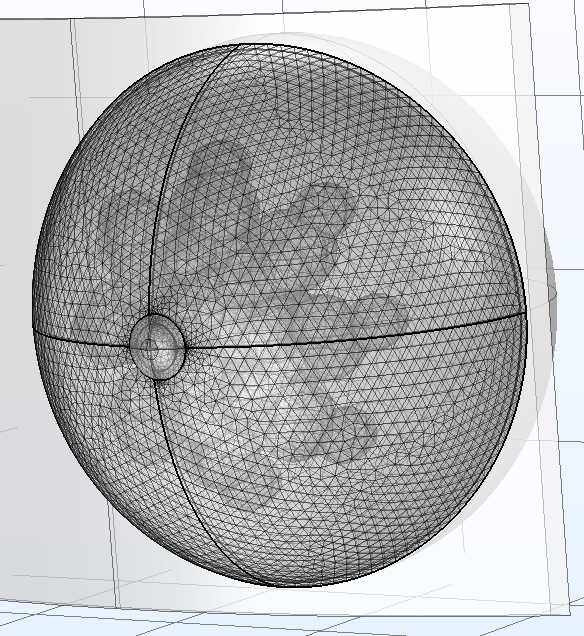
\includegraphics[width=0.45\linewidth]{Figures/M&M/report_mesh.png}
\caption{Example of the generated COMSOL tetrahedral mesh used for the breast model.}
\label{fig:comsol_mesh_example}
\end{figure}

The solver strategy consisted of a gravity-preload step followed by the time-dependent dynamic simulation. Build-only cases were used during development to verify generated selections and model setup before running full dynamic simulations.


%%%%%%%%%%%%%%%%%%%%%%%%%%%%%
% SECTION 3.6 BELOW
%%%%%%%%%%%%%%%%%%%%%%%%%%%%%


\subsection{Post-processing and evaluation metrics}
\label{post_processing_and_evaluation_metrics}

Post-processing was performed using the scripted COMSOL export and Python analysis workflow. For each completed simulation, compact output files were generated for displacement fields, selected stress quantities and time-dependent response measures. These outputs were used to evaluate how changes in model settings or parameter choices affected the simulated mechanical response, using the corresponding comparison case for each analysis.

Because the Early Warning Scan concept is based on observable breast-surface motion, the main evaluation focused on the free outer breast surface. In the COMSOL workflow this surface was represented by the \texttt{outer\_skin\_free\_bnd} selection. Whole volume displacement and stress measures were retained as supporting diagnostic quantities.

The displacement magnitude was defined as

\begin{equation}
u_{\mathrm{mag}}
=
\sqrt{u^{2}+v^{2}+w^{2}},
\label{displacement_magnitude_definition}
\end{equation}

where $u$, $v$ and $w$ are the displacement components in the $x$-, $y$- and $z$-directions. In addition to the magnitude, signed displacement components were evaluated because they preserve direction. The vertical displacement component $w$ was used to describe upward or downward surface motion during dynamic excitation.

For surface-based evaluation, spatial averages were computed over the evaluated surface selection $S$,

\begin{equation}
\bar{q}_{S}(t)
=
\frac{1}{A_{S}}
\int_{S} q(\mathbf{x},t)\,\mathrm{d}A,
\label{surface_average_metric}
\end{equation}

where $q$ is the evaluated displacement or stress quantity and $A_{S}$ is the surface area of the selection. For dynamic cases, signed vertical displacement was also evaluated relative to the dynamic-start state,

\begin{equation}
\Delta \bar{w}_{S}(t)
=
\bar{w}_{S}(t)
-
\bar{w}_{S}(t_{\mathrm{dyn,start}}).
\label{surface_vertical_displacement_from_dynamic_start}
\end{equation}

For prescribed support-displacement cases, the support-relative vertical displacement defined in Equation~\ref{support_relative_vertical_displacement} was used in addition to the absolute displacement. Landmark-patch displacements were also exported for selected surface regions, including the nipple and superior, inferior, left and right breast-surface patches. These patch-averaged values were used as robust surface-motion measures, because they are less sensitive to individual mesh nodes than single-point displacement values.

Stress was evaluated using the exported von Mises stress field. This was used as a mechanical diagnostic for comparing stress concentration between model variants. For the tumor cases, local displacement and stress measures were additionally evaluated using the tumor mask region.

COMSOL animations were also generated for qualitative inspection of the time-dependent deformation patterns. These animations were not used as quantitative evidence; the reported Results are based on the exported displacement, stress, surface and tumor-mask metrics. The post-processing quantities used for the main model comparisons are summarised in Table~\ref{post_processing_metrics_table}.

\begin{table}[H]
\centering
\small
\caption{Post-processing quantities used to compare COMSOL model variants.}
\label{post_processing_metrics_table}
\begin{tabular}{p{0.28\linewidth} p{0.32\linewidth} p{0.30\linewidth}}
\toprule
Quantity & Definition or source & Use in evaluation \\
\midrule
Free-surface displacement 
& $u$, $v$, $w$ and $u_{\mathrm{mag}}$ on \texttt{outer\_skin\_free\_bnd} 
& Main EWS-relevant surface-motion response. \\

Surface-average response 
& $\bar{q}_{S}(t)$ and $\Delta \bar{w}_{S}(t)$ 
& Average dynamic response of the visible breast surface. \\

Landmark-patch displacement 
& Patch-averaged displacement on nipple and breast-surface landmark selections 
& Robust comparison of visible local surface motion. \\

Support-relative displacement 
& $w_{\mathrm{rel}}=w-z_{\mathrm{support}}$ 
& Deformation relative to prescribed support motion. \\

von Mises stress 
& Exported COMSOL stress field 
& Mechanical stress-concentration diagnostic. \\

Tumor-region response 
& Mask-based displacement and stress measures 
& Local response around the analytic tumor overlay. \\

Peak response 
& Maximum value over the evaluated time range 
& Quantitative comparison between corresponding cases. \\
\bottomrule
\end{tabular}
\end{table}

When variants were compared, changes were reported relative to the corresponding comparison case,

\begin{equation}
\Delta q_{\%}
=
100
\frac{q_{\mathrm{variant}}-q_{\mathrm{comparison}}}{q_{\mathrm{comparison}}},
\label{relative_metric_difference}
\end{equation}

where $q$ denotes the evaluated displacement or stress metric. This percentage difference was used only when the comparison value was non-zero and physically meaningful.

%%%%%%%%%%%%%%%%%%%%%%%%%%%%%
% SECTION 3.7 BELOW
%%%%%%%%%%%%%%%%%%%%%%%%%%%%%


\subsection{Reproducibility and data management}
\label{reproducibility_and_data_management}

The project was organised to keep the COMSOL workflow reproducible and traceable. Source code, TOML case definitions, report notes and compact post-processing outputs were maintained in the project repository \cite{KuijpersEWSComsolGitHub}. Large generated files, such as full COMSOL model files, temporary solver files and extensive raw exports, were kept outside version control because they can be regenerated from the scripted case definitions.

Each COMSOL case was defined by a version-controlled TOML file. These files stored the relevant geometry route, material parameters, loading settings, mesh settings and output options for each model variant. The Python pipeline converted these case definitions into COMSOL Java builder scripts and post-processing outputs. This reduced manual editing in COMSOL and made it easier to inspect or rerun model variants.

The simulations were run using a licensed COMSOL Multiphysics installation available through TU/e. All model builds and time-dependent solves reported in this work were executed on local hardware during model development. The software and hardware environment used for the simulations is summarised in Table~\ref{software_hardware_environment_table}.

\begin{table}[H]
\centering
\small
\caption{Software and hardware environment used for COMSOL model development and simulation runs.}
\label{software_hardware_environment_table}
\begin{tabular}{p{0.32\linewidth} p{0.58\linewidth}}
\toprule
Item & Setting \\
\midrule
COMSOL version & COMSOL Multiphysics 6.4 \\
License environment & TU/e licensed COMSOL installation \\
Operating system & Windows 11 Enterprise \\
Processor & 11th Gen Intel Core i7-11800H, 2.30GHz \\
Memory & 16.0 GB RAM \\
Python environment & Python 3.8.8 \\
Repository & \cite{KuijpersEWSComsolGitHub} \\
\bottomrule
\end{tabular}
\end{table}
